\section{Clickstream data: Interface participants' time spent}
In addition to distance, we analyze the time participants spend per option. We aggregate the total time participants spend per option using the QS system log. For participants in the two-phase interface conditions, this includes both organization and voting times for that option. The results are visualized in Figure~\ref{fig:total_time}.


\begin{figure}[h]
    \centering
    % First subfigure
    \begin{subfigure}[b]{0.45\textwidth}
        \centering
        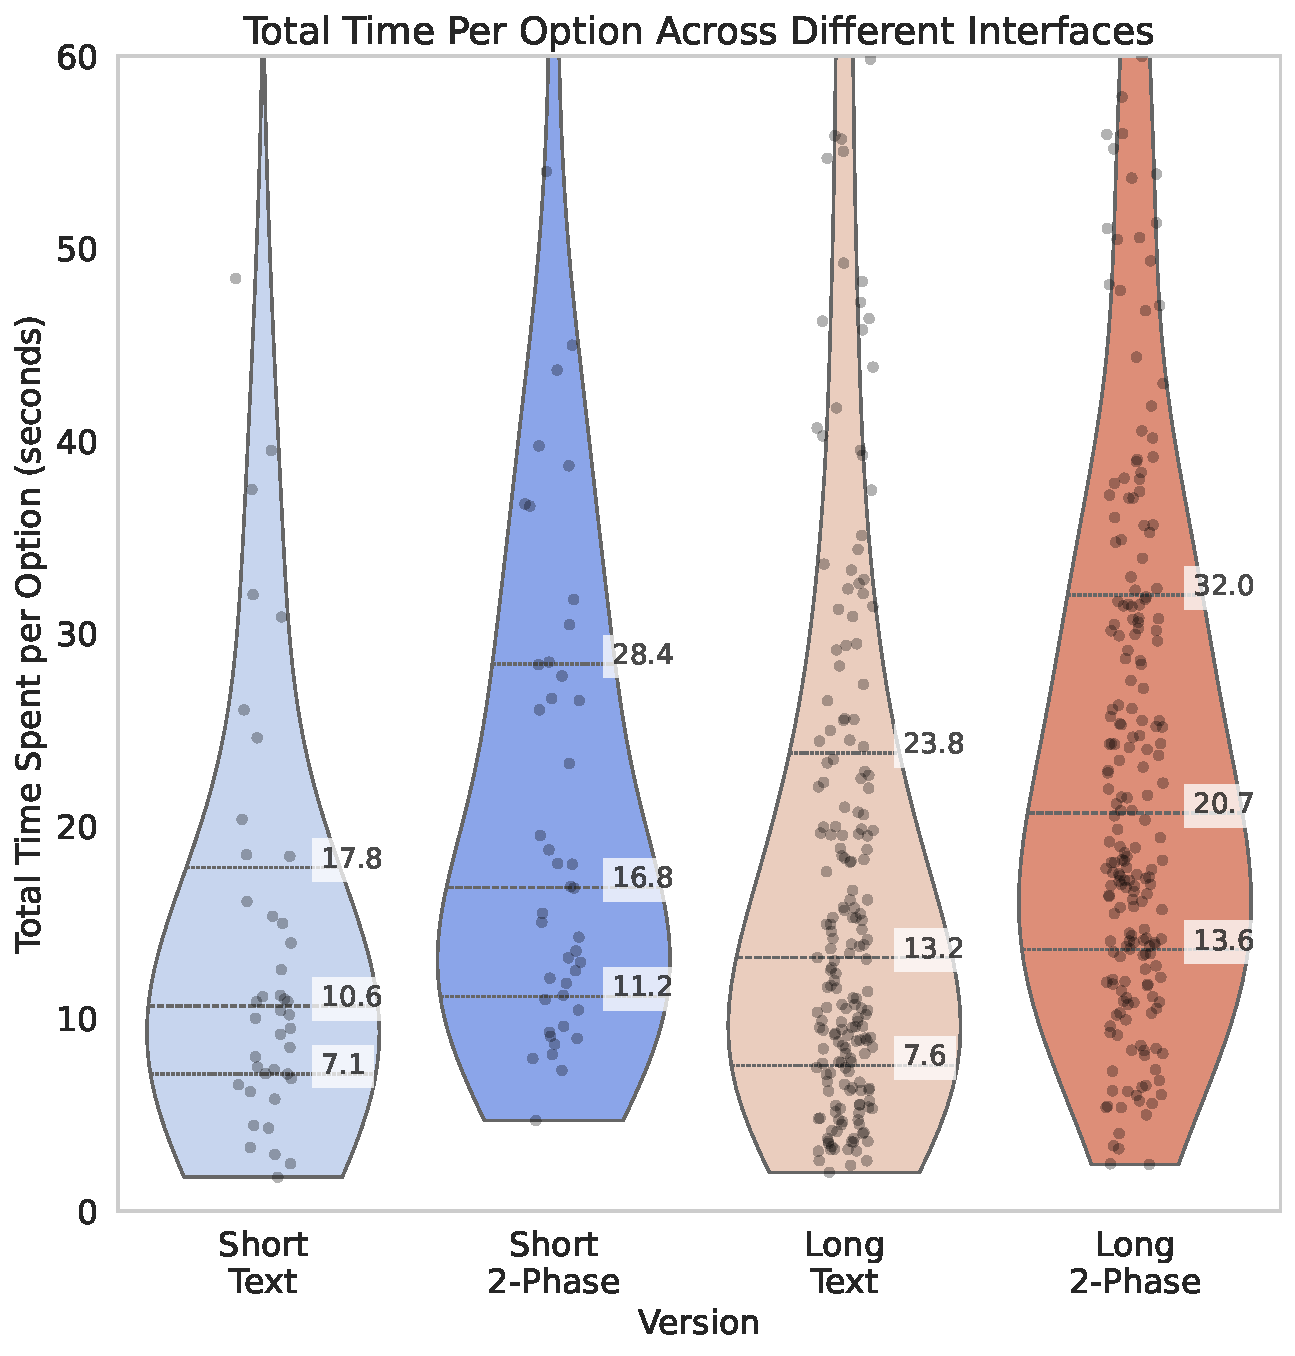
\includegraphics[width=0.95\textwidth, trim=0 0 0 0, clip]{content/image/time/Total Time Per Option Across Different Interfaces.pdf}
        \captionsetup{width=\textwidth, justification=justified} % Adjust the width to match the image width
        \caption{Total Time per option: We identified that the two-phase interface skewed slightly higher than the text interface, as expected. This discrepancy can be attributed to the extra organization step required in the two-phase interface, leading to a slightly longer overall completion time per option.}
        \Description{Violin plot showing total time spent per option in seconds across four interface versions: Short Text, Short 2-Phase, Long Text, and Long 2-Phase. The y-axis ranges from 0 to 60 seconds. Each violin plot has scattered dots representing individual data points. The shape of the Short Text plot is widest between 10 and 20 seconds, tapering at the top and bottom. The Short 2-Phase plot is the narrowest, with most dots concentrated between 10 and 20 seconds. The Long Text plot is narrow and widest near the bottom, between 5 and 15 seconds. The Long 2-Phase plot is widest near the top, between 20 and 40 seconds.}
        \label{fig:total_time}
    \end{subfigure}
    \hfill
    % Second subfigure
    \begin{subfigure}[b]{0.45\textwidth}
        \centering
        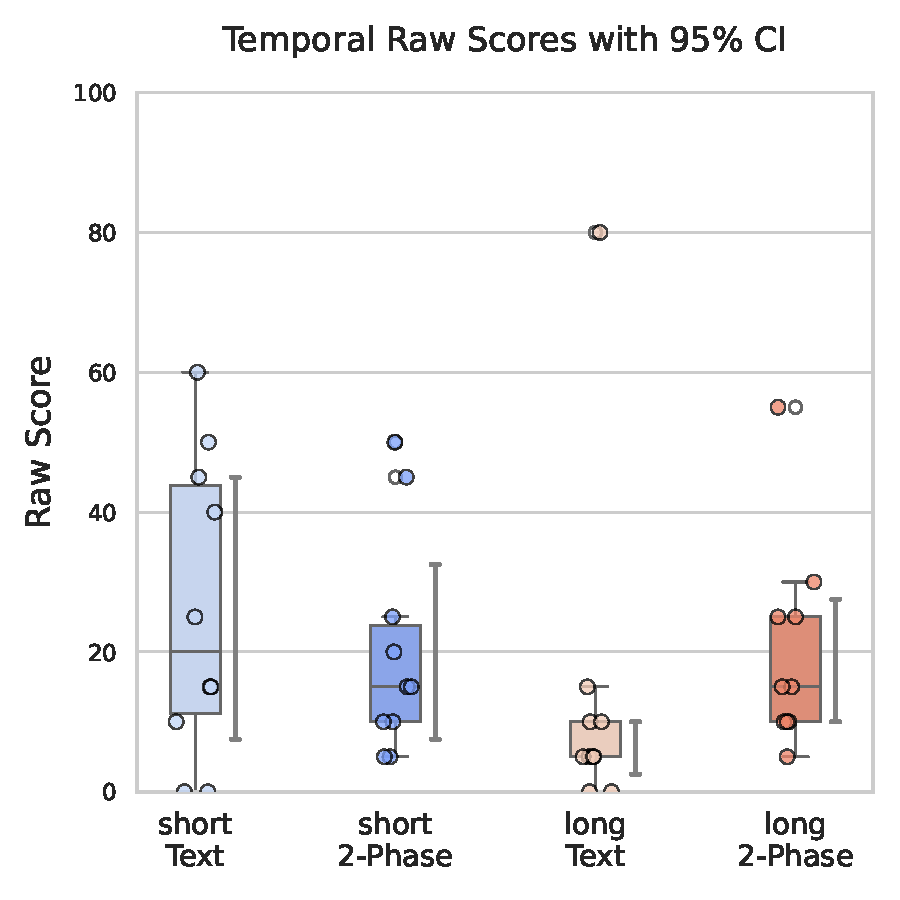
\includegraphics[width=0.95\textwidth, trim=0 13 0 13, clip]{content/image/cog/Temporal_scores.pdf}
        \captionsetup{width=\textwidth, justification=justified} % Adjust the width to match the image width
        \caption{Temporal Demand Raw Score: The short text interface results in the highest temporal demand, while the long text interface is the lowest. Two-phase interfaces show moderate temporal demand, suggesting that interactive elements allowed participants to pace themselves better.}
        \label{fig:temporal_cog_score}
    \end{subfigure}
\end{figure}

\begin{figure}[ht]
    \centering
    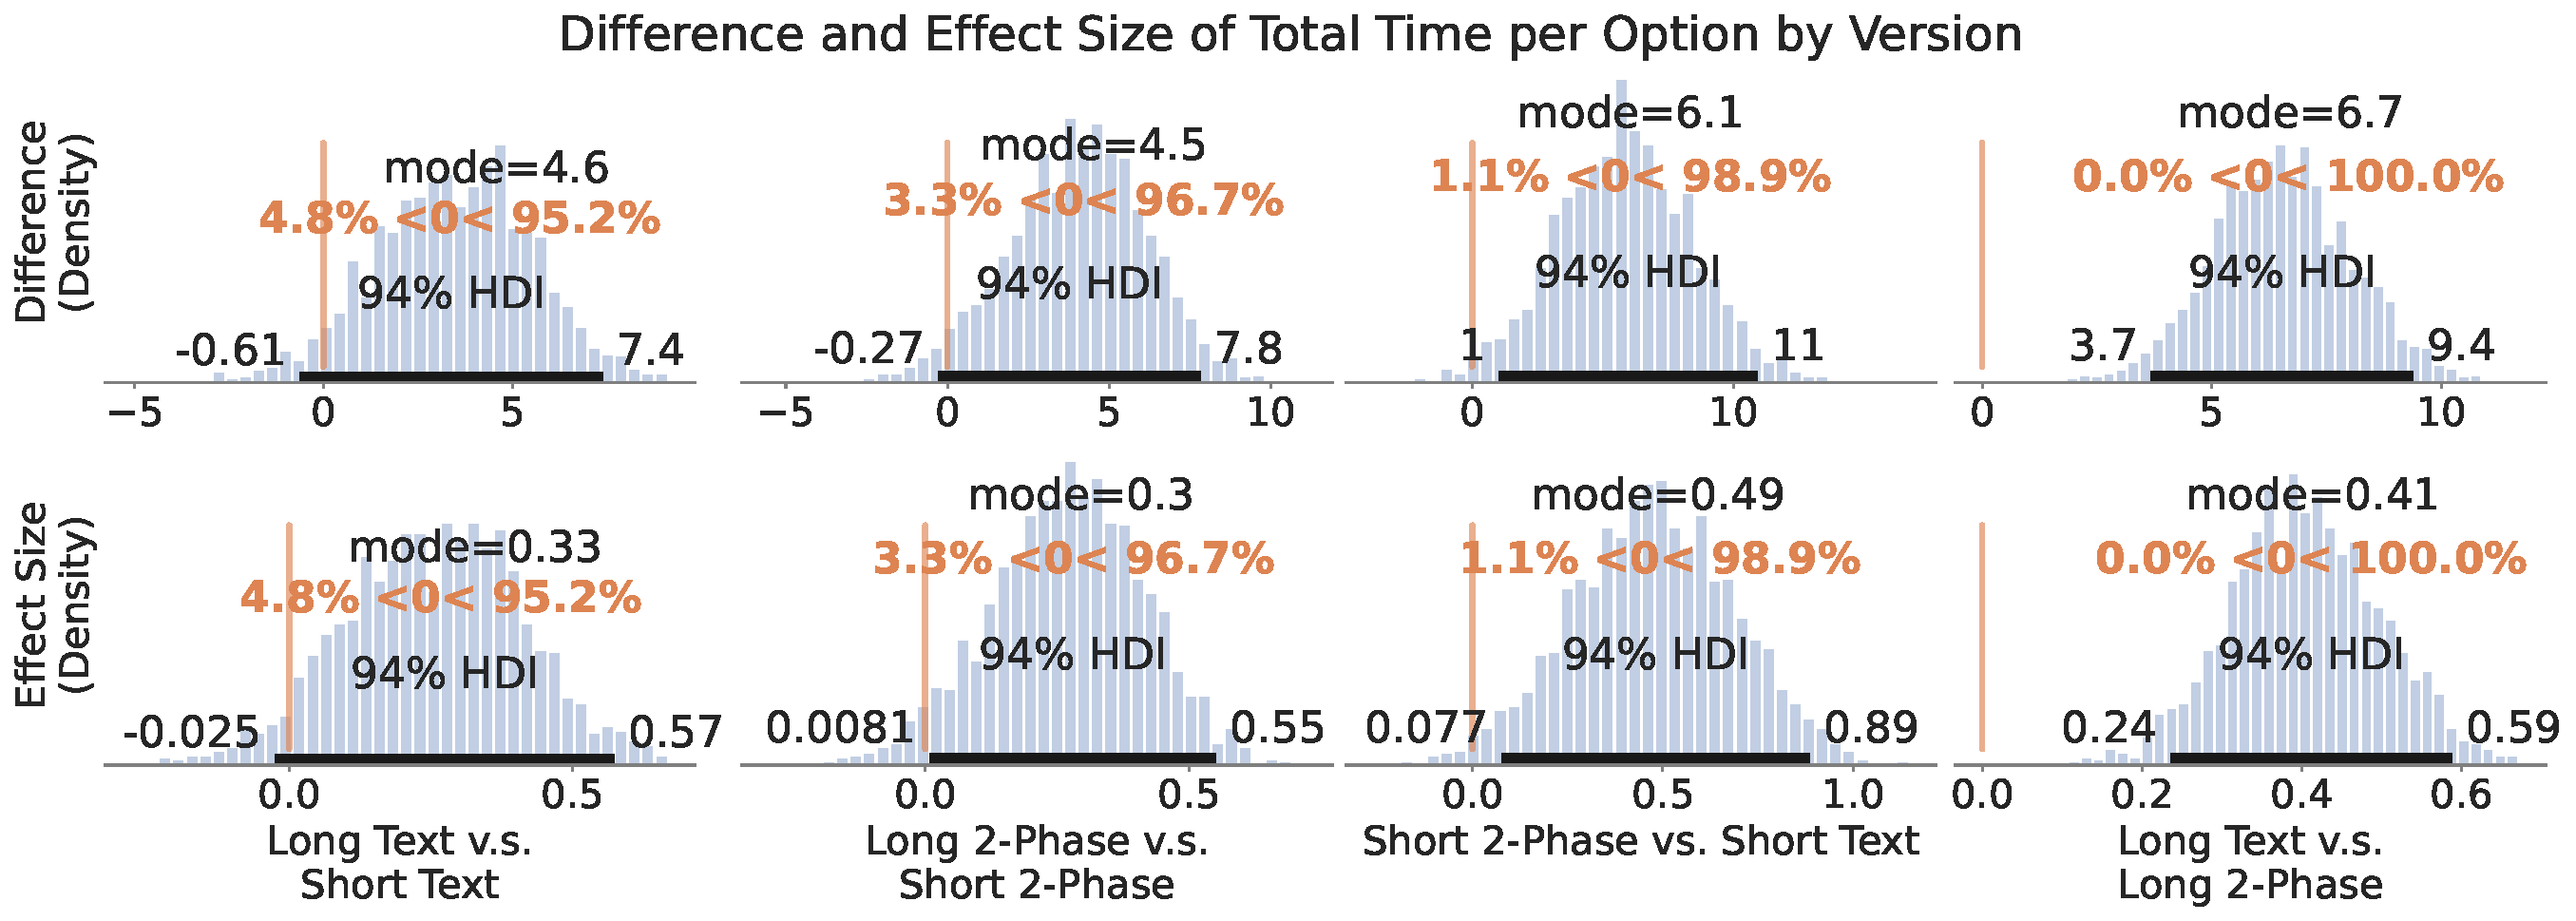
\includegraphics[width=0.8\textwidth]{content/image/time/time_diff_per_option_effect_size_by_version}
    \caption{Bayesian Time Diff}
    \label{fig:time_per_option_bayesian}
\end{figure}

Overall, participants spend slightly more time per option in the two-phase interface than in the text interface. To quantify these observations, we model the time data as predictive variables of separate Gamma distributions to characterize the continuous response times observed under distinct experimental conditions defined by survey length and interface type. Each of the four resulting subsets of data is modeled independently, with separate Gamma-distributed parameters governing the shape and rate of each group's time distributions. 

We calculated the posterior differences between the two-phase and text interfaces for all pairwise comparisons of the four groups. The results in Figure~\ref{fig:time_per_option_bayesian} indicate that participants using the two-phase interface consistently spend more time per option than those using the text interface, regardless of survey length. For both the short and long QS, participants most likely spend 6.1 seconds (94\% HDI = [1.0, 11.0]) and 6.7 seconds (94\% HDI = [3.7, 9.4]) more per option, respectively, with medium effect sizes of $d=0.49$ (94\% HDI = [0.077, 0.89]) and $d=0.41$ (94\% HDI = [0.24, 0.59]). In both cases, the intervals lie outside the ROPE of 0 ± 1, indicating statistical significance. These findings suggest that the two-phase interface encourages longer deliberation, particularly for longer lists of options. Details of the model are provided in Appendix XX.

Some literature points to increased time leading to time fatigue~\cite{}, which can impair decision-making. Other decision science literature suggests that longer decision times can indicate deeper cognitive processing~\cite{payneAdaptiveDecisionMaker1993}. Our qualitative analysis points to the latter.

Other than the difference in operational thinking and strategic consideration discussed in Section~\ref{sec:demand}, we find that 37.5\% of participants (N=15) who attribute time to \textit{Decision Making} as a source of temporal demand frame such demand differently. We label a participant as \textit{affirmative} if they describe the pressure to make decisions as a source of temporal demand. For example, \smallquote{S022}{So it didn't take too much time, but obviously there were a lot of things to consider, so there was some temporal demand.} is an affirmative statement. Conversely, we label a participant as \textit{negative} if they express concern about the time and effort they have already invested. For example, \smallquote{S024}{maybe I should just hurry up and make a decision.} is a negative statement.

50\% of participants (N=5) in the long two-phase group describe the pressure to make decisions affirmatively and none negatively. This suggests that their pressure stems from having too many remaining decisions to make, rather than from the time already invested. This is reflected in their higher average time spent per option and overall time spent ($\mu=716.86$ seconds, $\sigma=164.04$ seconds) completing the QS survey compared to the long text group ($\mu=449.64$ seconds, $\sigma=206.97$ seconds). We interpret this as evidence that participants are thoughtfully engaged in constructing their preferences and choose to invest additional time, rather than being driven by decision-related pressures or experiencing a sense of urgency.

Conversely, in the short text group, 50\% of participants (N=5) express concern about the time and effort they have already invested~(\smallquote{S024}{maybe I should just hurry up and make a decision.}) and none frame it affirmatively. Descriptively, participants in the short text group spend comparatively less time than those in the long QS (short text: $\mu=139.83$ seconds, $\sigma=76.43$ seconds; short two-phase: $\mu=178.78$ seconds, $\sigma=61.07$ seconds). This suggests that participants in the short text group expect themselves to complete the task sooner than they actually do. 

Surprisingly, participants in the long text interface exhibit a temporal demand lower than the short text and long 2-phase participants(Figure~\ref{fig:temporal_cog_score}, quantifiable results in Appendix XX), despite spending more time per option and traversing the longest distance (Section~\ref{sec:dist}). Only 30\% of participants (N=3) mention the time spent making a decision as a source of temporal demand. One possible explanation is that some participants are satisficing, which we will discuss further in Section~\ref{ref:secsatisfice}.  

In summary, we interpret the result that participants in the two-phase interface spend more time per option as a sign of deeper cognitive processing. This is further supported by examining participants' nuanced voting behaviors under budget constraint conditions for the long QS, which we omit for brevity. Notably, two-phase interface participants make more small vote adjustments (i.e., adding or removing at most 2 votes on an option) when they have fewer remaining credits, further supporting our claim that they experience deeper engagement with preference construction, which we elaborate on further in Appendix~\ref{apdx:budget_voting_behaviors}.
